
\section{Laplace Transform}

$X(s) = \int_{-\infty}^{\infty} x(t) e^{-st} \rd  t$

Unilateral: $\int_{0-}^{\infty}$

\subsection*{Properties}

\emph{Reduced} rational fraction $X(s) = \frac{N(s)}{D(s)}$ (When $s=\infty$ is zero or pole)
% $\int_{-\infty}^{+\infty} e^{-st} e^{-\alpha t} u(t) \rd t = \frac{1}{a+s}(\Re{s}>-a)\\\int_{-\infty}^{+\infty} e^{-st} (-e^{-\alpha t}) u(-t) \rd t = \frac{1}{a+s}(\Re{s}<-a)$

\subsection*{ROC}

Right sided:$(\sigma \in \roc) \to (\Re{s}>\sigma \subseteq \roc)$

Left sided:$(\sigma \in \roc) \to (\Re{s}<\sigma \subseteq \roc)$

Two sided: $\sigma_1<\Re s<\sigma_2$

Bounded by poles or $\infty$, no poles contained in $\roc$

\subsection*{ILT}

$X(s)=\mathcal F\{x(t)e^{-\sigma t}\}\to x(t)=\frac{1}{2\pi j} \int_{\sigma-j\infty}^{\sigma+j\infty} X(s) e^{st}\rd t \\ = \frac{e^{\sigma t}}{2\pi}\int_{-\infty}^{+\infty} X(\sigma + j\om) e^{j\om t}\rd \om$ (when $\Re s =\sigma$ in $\roc$)

$\mathcal L^{-1}\{s^n\} = u_n(t), all~s$

$\mathcal L^{-1}\{\frac{1}{(s+a)^n}\} = \begin{cases} \frac{-t^{n-1}}{(n-1)!}e^{-at}u(-t), & \Re s <-a\\ \frac{t^{n-1}}{(n-1)!}e^{-at}u(t), & \Re s >-a\end{cases}$

\subsection*{Properties(ROC)}

$X_1(s)=\mathcal L\{ x_1(t)\},\roc=R_1 \\ X_2(s)=\mathcal L\{ x_2(t)\},\roc=R_2$

$aX_1(s) + bX_2(s) = \mathcal L\{ax_1(t) + bx_2(t)\}, \roc\supseteq R_1\cap R_2 $ 
($R_1\cap R_2=\emptyset\to \roc=\emptyset$)

$X_1^*(s^*)=\mathcal L\{x_1^*(t)\}, \roc=R_1$

$e^{-s\tau}X_1(s)=\mathcal L\{x_1(t-\tau)\}, \roc=R_1$

$X_1(s-\tau)=\mathcal L\{x_1(t)e^{\tau t}\}, \roc=R_1+\Re{\tau}$

$\frac{1}{|a|}X_1(\frac s a)=\mathcal L\{x_1(at)\}, \roc=aR_1=\{s|\frac s a \in R_1\}$

$X_1(s)X_2(s)=\mathcal L\{x_1(t) * x_2(t) \}, \roc \supseteq R_1\cap R_2$ (This equality may not hold if $R_1\cap R_2=\emptyset$)

$sX(s)=\mathcal L\{x'(t)\}, \roc \supseteq R_1, X'(s)=\mathcal L\{-tx(t)\}, \roc = R_1$

$\frac 1 sX(s)=\mathcal L\{\int_{-\infty}^t x(\tau)\rd \tau\}, \roc \supseteq (R\cap (\Re s>0))$

\subsection*{Examples}

$\mathcal L\{\cos(\om_0 t) u(t)\} = \frac{s}{s^2+\om_0^2}, \mathcal L\{\sin(\om_0 t) u(t)\} = \frac{\om_0}{s^2+\om_0^2}$

\subsection*{Analysis}

Casual $\to\roc=$ right-half plane

Casual(Rational) $\leftrightarrow\roc=$ right-half plane

LTI Stability $\leftrightarrow j\om-\text{axis}\subseteq\roc$

Casual Stability $\leftrightarrow$ all poles have negative real part 

\subsection*{Block Diagram}

Direct: $H(s) = \frac{\sum b_is^i}{\sum a_is^i}$, 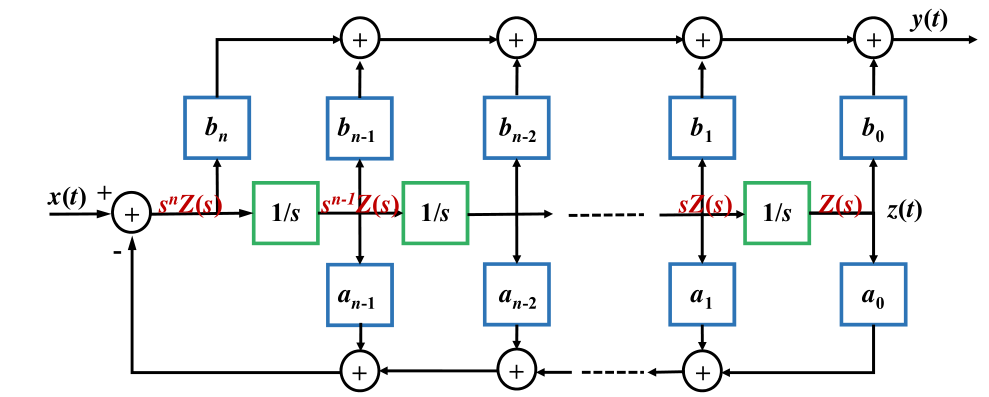
\includegraphics[scale=0.2]{inhalt/direct.png}

Parrallel: $H(s)=A\frac{\prod s-\alpha_i}{\prod s - \beta_i}$ 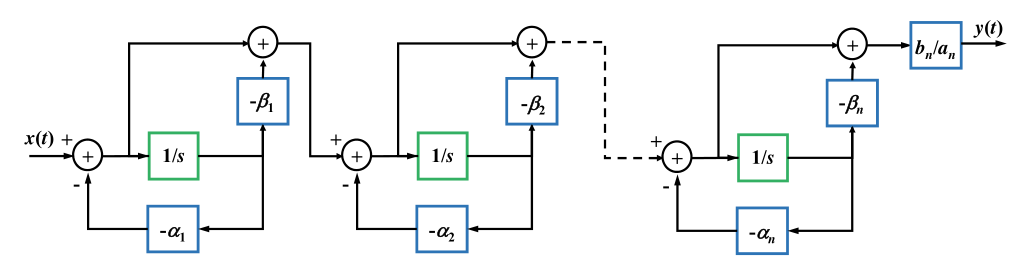
\includegraphics[scale=0.2]{inhalt/Parallel.png}

Cascade: $H(s) = \sum \frac{A_i}{s-a_i}$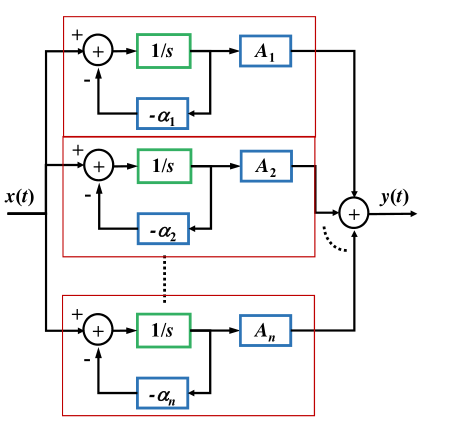
\includegraphics[scale=0.2]{inhalt/cascade.png}

\subsection*{Unilateral Laplace}